\documentclass[a4paper, 12pt, twoside]{article}
\usepackage[utf8]{inputenc}		% LaTeX, comprend les accents !
\usepackage[T1]{fontenc}		
\usepackage[francais]{babel}
\usepackage{lmodern}
\usepackage{ae,aecompl}
\usepackage[top=2.5cm, bottom=2cm, 
			left=3cm, right=2.5cm,
			headheight=15pt]{geometry}
\usepackage{graphicx}
\usepackage{eso-pic}	
\usepackage{array}	
\makeatletter
\def\@ecole{école}
\newcommand{\ecole}[1]{
  \def\@ecole{#1}
}
\def\@domaine{}
\newcommand{\domaine}[1]{
  \def\@domaine{#1}
}

\def\@specialite{Spécialité}
\newcommand{\specialite}[1]{
  \def\@specialite{#1}
}


\def\@master{Master}
\newcommand{\master}[1]{
  \def\@master{#1}
}

\def\@adresse{Adresse}
\newcommand{\adresse}[1]{
  \def\@adresse{#1}
}

\def\@encadranta{}
\newcommand{\encadranta}[1]{
  \def\@encadranta{#1}
}

\def\@encadrantb{}
\newcommand{\encadrantb}[1]{
  \def\@encadrantb{#1}
}
\def\@auteura{}{}{}
\newcommand{\auteura}[1]{
  \def\@auteura{#1}
}
\def\@auteurb{}{}{}
\newcommand{\auteurb}[1]{
  \def\@auteurb{#1}
}
\def\@auteurc{}{}{}
\newcommand{\auteurc}[1]{
  \def\@auteurc{#1}
}
\def\@auteurd{}{}{}
\newcommand{\auteurd}[1]{
  \def\@auteurd{#1}
}
\makeatother




\makeatletter
\newcommand{\pagedegarde}{
\newgeometry{top=2.5cm, bottom=1cm, left=2cm, right=1cm}
  \begin{titlepage}
  \centering
      
\includegraphics[width=1\textwidth]{limogelogo.pdf}
    \vspace{1cm}
      {\huge 
    \vspace{0.5cm}
        {\huge\bfseries \@ecole}\\
    \vspace{0.2cm}
        {\Large\bfseries \@domaine}\\
    \vspace{0.5cm}
        {\Large\bfseries Master 1 }\\
    \vspace{0.2cm}
        {\large\bfseries Sécurité informatique et cryptologie }\\
    \vspace{1cm}
    	MEMOIRE DU SECOND SEMESTRE}\\
    \vfill
       {\LARGE \color[rgb]{0,0,1} \bfseries{\@title}} \\
    \vspace{2cm}
    	{\bfseries \@auteura}\\
    	{\bfseries \@auteurb}\\
    	{\bfseries \@auteurc}\\
    	{\bfseries \@auteurd}\\
    \vspace{0.5cm}
        Encadrants :\\
        {\bfseries \@encadranta}\\
        {\bfseries \@encadrantb}\\
    \vspace{0.5cm}
        {\Large\bfseries \@date}\\
    \vfill
  \end{titlepage}
\restoregeometry
}
\author{}
\auteura{Thanina \textsc{Alili}}
\auteurb{Thibault \textsc{Debonnière}}
\auteurc{Baptiste \textsc{Decrand}}
\auteurd{Ndiasse \textsc{Thioune}}
\title{Analyse Forensic d'un Ransomware}
\master{Master 1 Informatique}
\specialite{CRYPTIS}
\encadranta{Jean-Louis \textsc{Lanet}}
\encadrantb{Benoit \textsc{Crepin}}
\date{Novembre 2017}
\ecole{UNIVERSIT\'{E} DE LIMOGES}
\domaine{
	\textbf{FACULT\'{E} DES SCIENCES ET TECHNIQUES}
}
\begin{document}
\pagedegarde
\tableofcontents
\newpage
\section{Introduction}
\subsection{Contexte}
Dans le cadre de la validation de la première année master informatique à l’université de Limoges, nous avons choisi le projet Analyse forensic d’un ransomware.
\subsection{Intérêts du document}
Ce document présente les différents objectifs et étapes de l'application, il sera le plus détaillé possible de manière à être en accord sur les choix et besoins de l'application pour notre mémoire.
\subsection{Présentation de l'application}
Ce projet a pour but de réaliser une application qui permet depuis une image mémoire d’un ransomware de retrouver la famille à laquelle il appartient. L'utilisateur  pourra ainsi proposer ces images mémoires depuis une interface graphique afin d'obtenir leurs classifications. Cette application sera réalisée en deux temps, un prototype sera créé au cours du premier semestre ne contenant qu’une seule métrique tandis que la version finale qui sera implémentée au cours du second semestre comportera huit métriques en tout.
\subsection{Critères d'acceptabilité}
L'application sera acceptée si elle répond aux critères suivants:
\begin{itemize}
\item L'application respecte les contraintes clients.
\item L'application respecte les contraintes techniques.
\item L'application suit les spécifications du cahier des charges.
\item L'application présente les principales fonctionnalités évoquées.
\end{itemize}
\section{Expression du besoin}
\subsection{Acteurs}
L’utilisateur de l’application est considéré comme l’unique acteur de celle-ci. Aucune configuration réseau ou de lien avec d'autres applications n'est prévue.
\subsection{Scénario d'utilisation}
\large Scénario de l'utilisateur:
au moment où l'utilisateur lance l'application, une interface graphique apparaît et lui propose de classifier un ransomware, l'utilisateur a alors la possibilité d'indiquer le chemin du fichier au programme et les métriques à utiliser, afin de rechercher une classification l'utilisateur clique sur le bouton "classifier". Une fois l'algorithme fini, l'interface graphique indique ces résultats.
L'utilisateur peut alors proposer à nouveau une image mémoire ou bien quitter l'application.
\subsection{Fonctionnalités}
\begin{tabular}{|l|l|}
    \hline
   Fonctionnalités & Description\\
   \hline
   FP01 & Démarrer\\
   \hline
   FP02 & Quitter\\
   \hline
   FS01 & Indiquer l'emplacement d'un fichier mémoire\\
   \hline
   FS02 & Choisir les métriques à utiliser\\
   \hline
   FS03 & Rechercher la classification du fichier mémoire\\
   \hline
   FS04 & Rechercher une clé de chiffrement\\
   \hline
   FS05 & Consulter les résultats de la classification\\
   \hline
\end{tabular}\\
\paragraph{}
{\bfseries FP01: Démarrer}\\
Ouvre une fenêtre graphique permettant à l'utilisateur de tester ces fichiers mémoire.
\paragraph{}
{\bfseries FP02: Quitter}\\
Quitte l'application via la croix de fermeture de la fenêtre.
\paragraph{}
{\bfseries FS01 : Indiquer l'emplacement d'un fichier mémoire}\\
En cliquant sur un bouton parcourir, le client pourra parcourir ces espaces de stockages et sélectionner le fichier mémoire à étudier.
\paragraph{}
{\bfseries FS02: Choisir les métriques à utiliser}\\
L'utilisateur sélectionnera une ou plusieurs métriques à l'aide d'un système de checkbox; une checkbox permettra de sélectionner l'ensemble des métriques.
\paragraph{}
{\bfseries FS03: Rechercher la classification du fichier mémoire}\\
L'utilisateur lancera l'algorithme à l'aide du bouton "Recherche", celui-ci en fonction des métriques choisis, étudiera le fichier mémoire de l'utilisateur et retournera les résultats.
\paragraph{}
{\bfseries FS04: Rechercher une clé de chiffrement}\\
L'utilisateur lancera un algorithme à l'aide du bouton "Recherche de clé de chiffrement", celui-ci étudiera le fichier mémoire de l'utilisateur et retournera les résultats indiquant les potentiels clés si il y'en a sinon il signalera un échec de la recherche.
\paragraph{}
{\bfseries FS05: Consulter les résultats de la classification}\\
Une fois la recherche terminé, l'utilisateur pourra consulter les résultats à travers l'interface graphique qui affichera le taux de ressemblance suivant chaque métrique et famille de ransomware.
\section{Contrainte}
\subsection{Contraintes Techniques}
L’analyse se fait sur un grand nombre de données. L’application devra être optimisée notamment sur les algorithmes de métrique afin qu’aucun ralentissement n’irrite l’utilisateur. L’application pourra fonctionner sur n’importe quel OS.

\subsection{Contraintes client}
L’application devra récupérer les chaînes de caractères et les transformées en vecteurs binaires

L’application utilisera huit métriques de distance 

L’application devra contenir une interface graphique permettant à l’utilisateur de proposer des fichiers mémoires à étudier et de consulter les résultats.
L’application devra détecter et enregistrer les clés de chiffrement et les librairies utilisées par le ransomware.

\section{Risques}
La réalisation du projet implique les risques suivants:
Le non-respect des délais.
L’application peut posséder des bugs recensés ou encore inconnus.
L’application peut avoir un dysfonctionnement sur certains ordinateurs en fonction des droits de l’utilisateur ou bien de la version du système et de Java.
L’application peut être sensible sur certains systèmes dont l’état est instable (disque dur plein, mémoire vive faible etc).

La catégorisation par apprentissage n’est pas une science exacte : SI les sources d’apprentissage s’avèrent fausse, les résultats suivants seront erronés et ne correspondront pas à la finalité souhaitée.

\section{Livrables}
Documents:
\begin{itemize}
\item Un cahier des charges en accord avec M. Jean-Louis lanet
\item Un dossier de conception qui définira la structure du projet
\item Un manuel d’utilisateur
\item L’ensemble des sources du projet
\item L’application compilé
\end{itemize}
Une présentation de l’application sera faite lors de la soutenance à la fin du deuxième semestre

\section{Annexes}
\subsection{Diagramme de Gantt}
\centering
      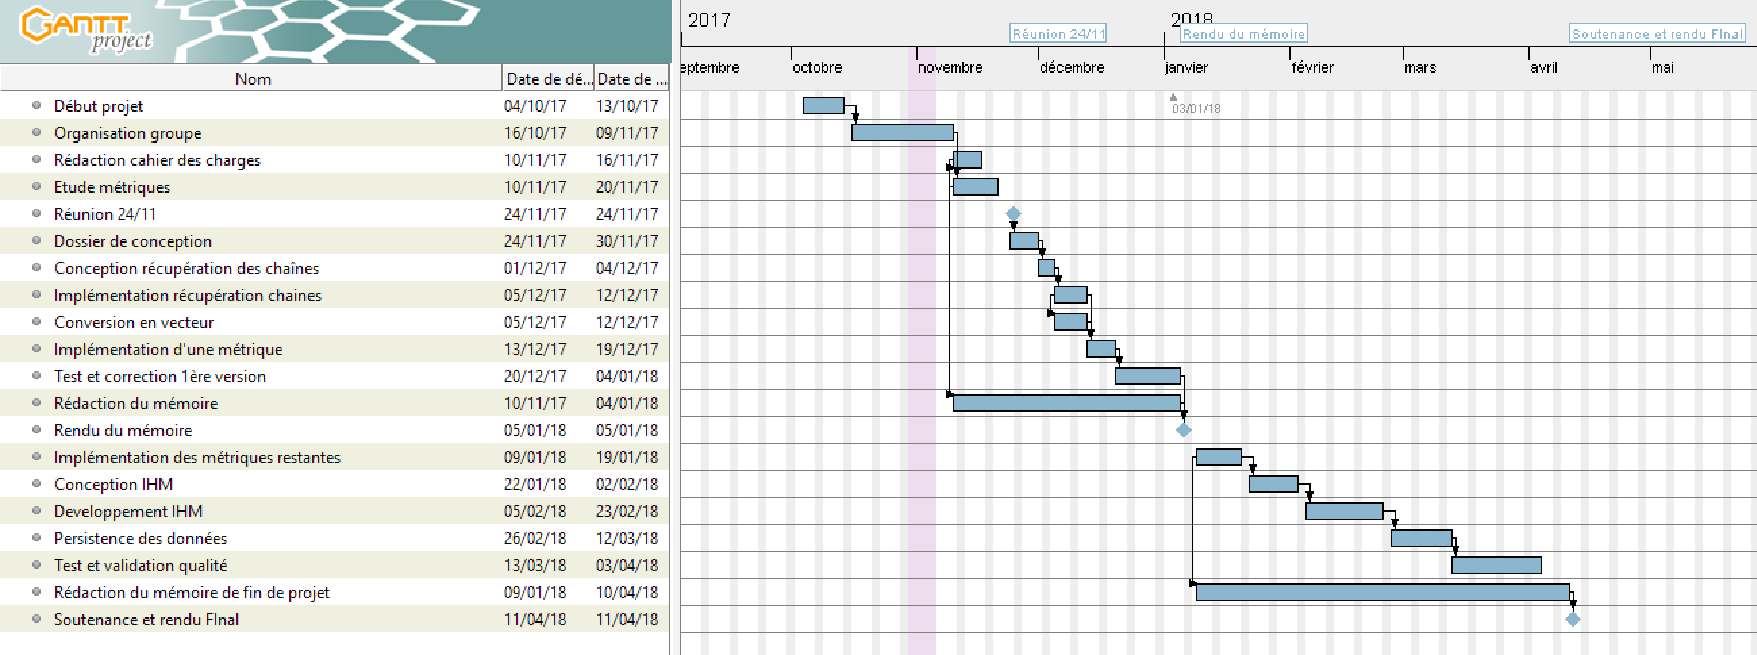
\includegraphics[width=1\textwidth]{gantt(1).pdf}
\subsection{Diagramme de PERT}
\centering
      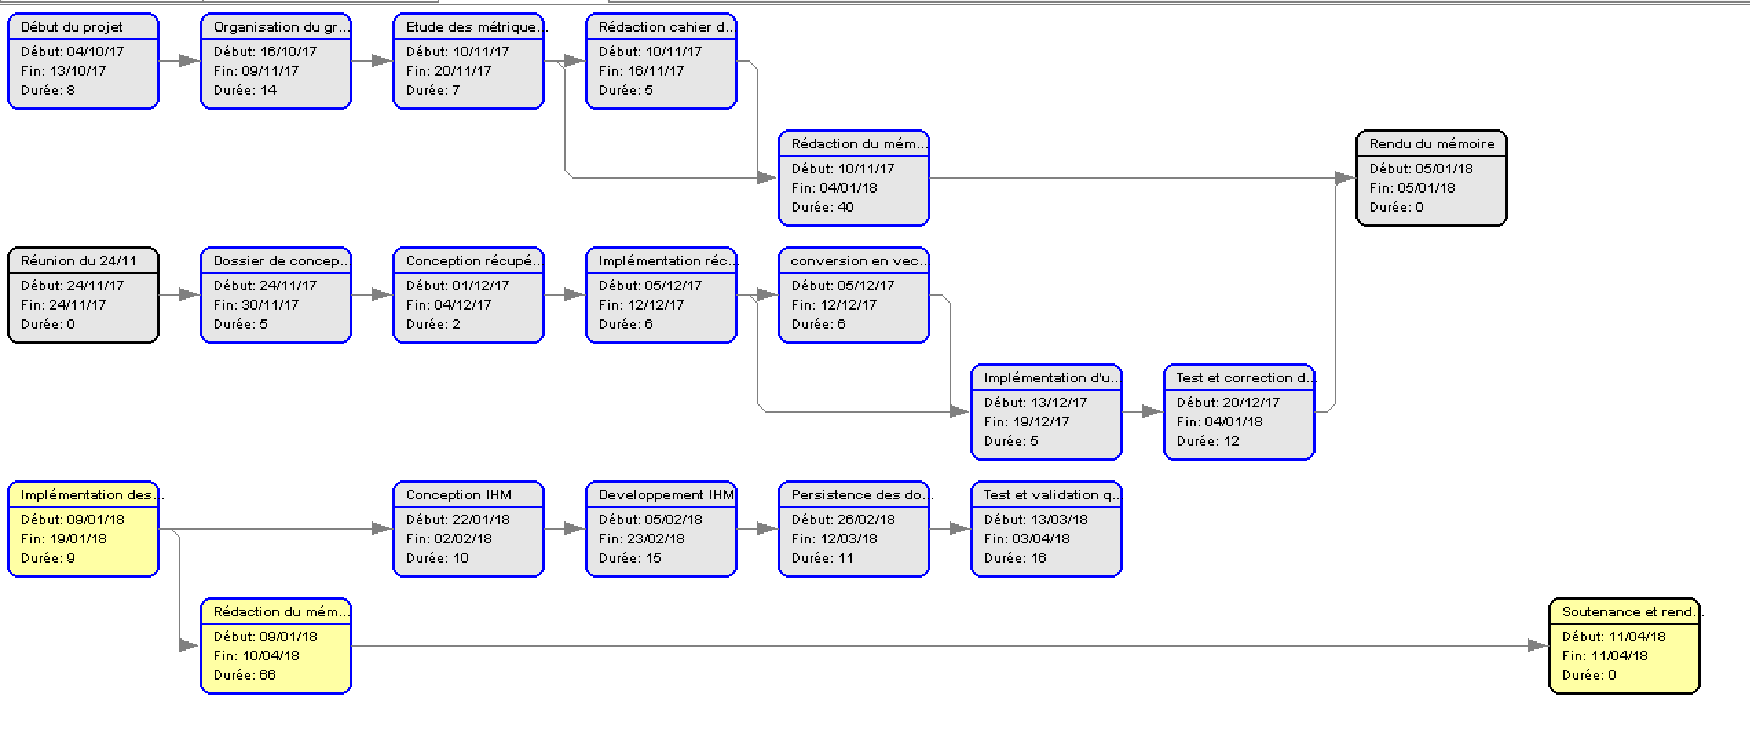
\includegraphics[width=1\textwidth]{pert(1)(1).pdf}


% Et tout le reste du document
\end{document}